% Lenguajes de Programación 2019-1
% Plantilla para reportes de laboratorio.

\documentclass{article}

\usepackage{authblk}
\usepackage[spanish]{babel}
\usepackage[utf8]{inputenc}
\usepackage{listings}
\usepackage{enumerate}
\usepackage{graphicx}


\title{Práctica 5}
\author{Galeana Araujo Emiliano (No. de Cuenta: 314340520)\\}
\author{Miranda Sánchez Kevin Ricardo (No. de Cuenta: 314011163)}\affil{Facultad de Ciencias, UNAM}
\date{28 Noviembre 2018}

\begin{document}

\maketitle

En esta práctica se desarrollaron dos temas vistos en clase cuales son \textbf{Excepciones} y \textbf{Continuaciones}. 
Y se modifico el ultimo semanal de modo que pudiéramos crear 3 módulos. Estos son: \newline
\begin{enumerate}
    \item FEAB. Aquí la forma más simple de una excepción es un error que no tiene información asociada. Este error se puede interceptar y convertir en un cómputo correcto transfiriendo el control a otra expresión. Haciendo uso de las \textbf{Catch Expr Expr} y \textbf{Error} como extensión del lenguaje EAB que siguen la semántica dinámica: \newline
    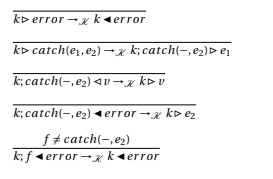
\includegraphics[scale=0.5]{1}
    \item XEAB. Aquí el argumento de la expresión \textbf{Raise} se evaluará para determinar el valor que se pasará al manejador. La expresión \textbf{Handle} liga la variable x a la expresión manejadora. El valor asociado de la excepción estará ligado en la expresión manejadora en caso de que se genere una excepción cuando se evalúa la primera expresión.\newline
    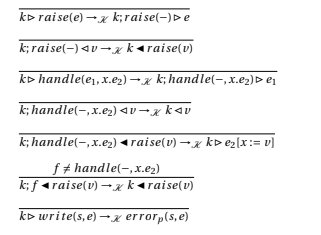
\includegraphics[scale=0.5]{4}
    \item KEAB.Aquí la idea para las continuaciones es considerar a la pila de control de un programa como un valor el cual puede devolverse o pasarse como argumento a otra función.\newline
    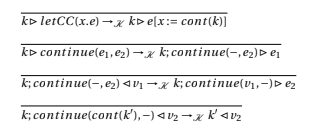
\includegraphics[scale=0.5]{6}

\end{enumerate}


\section{Entrada y ejecución}
Para ejecutar el programa se debe estar ubicado el directorio src, abrir una terminal y escribir \textbf{ghci $<$archvio$>$.hs} donde archivo debe ser elegido entre FEAB.hs, XEAB.hs y KEAB.hs, inmediatamente después debe aparecer:\newline
\begin{lstlisting}[language=Haskell]
GHCi, version 7.10.3: http://www.haskell.org/ghc/  :? for help
[1 of 1] Compiling KEAB             ( KEAB.hs, interpreted )
Ok, modules loaded: KEAB.
*KEAB>

\end{lstlisting}\newline
Como ejemplo del programa del archivo KEAB.hs: 
\begin{lstlisting}[language=Haskell]
*KEAB> eval (LetCC "k"(Succ (Continue (V "k")(Continue (V "k") (I 1)))))
N[1]
\end{lstlisting}
Como ejemplo del programa del archivo XEAB.hs: 
\begin{lstlisting}[language=Haskell]
*XEAB> eval (Handle (Add ( Let "x" (I 0) (If(Eq(I 0)(I 0))
(Raise(I 10))(Add(I 9)(V "x"))))(I(-1)))"h"(Mul(I 2)(V "h" )))
N[20]
\end{lstlisting}
Como ejemplo del programa del archivo FEAB.hs: 
\begin{lstlisting}[language=Haskell]
*FEAB> v t [] (Add (I 1) (Suc Error)) Integer
True
\end{lstlisting}

\section{Conclusiones}
Fue complicado programarlos, es notable la diferencia entre las definiciones teóricas y la implementación ya que para algunas funciones se debía encontrar algunos casos especiales.
Por otro lado, el separar los temas y crear nuevos módulos nos ayudo a un mejor entendimiento de los temas.

%Bibliografia

\begin{thebibliography}{9}

\bibitem{lamport94}
  lp191n12.pdf, lp191n13.pdf, Archivero, curso de Lenguajes de Programacion 2019-1.
\end{thebibliography}

\end{document}